\documentclass[12pt]{article}
\usepackage{amsfonts, epsfig}


\usepackage{graphicx}
\usepackage{fancyhdr}
\pagestyle{fancy}
\lfoot{\texttt{coms30127.github.io}}
\lhead{Computation Neuroscience - 03.4\_perceptron - Conor}
\rhead{\thepage}
\cfoot{}

\usepackage{graphicx}

\usepackage{listings}

\usepackage{tikz}

\usepackage{pgf}
\usepackage[utf8]{inputenc}
\usetikzlibrary{arrows,automata}
\usetikzlibrary{positioning}


\tikzset{
    state/.style={
           rectangle,
           rounded corners,
           draw=black, very thick,
           inner sep=2pt,
           text centered,
           },
}
\tikzset{
    on/.style={
           circle,
           draw=red, very thick,
           inner sep=2pt,
           fill=red!25,
           },
}


\tikzset{
    off/.style={
           circle,
           draw=blue, very thick,
           inner sep=2pt,
           text centered,
           },
}



\tikzset{
    neuron/.style={
           rectangle,
           rounded corners,
           draw=black, very thick,
           inner sep=2pt,
           text centered,
           },
}



\tikzset{
    area/.style={
           rectangle,
           draw=black, very thick,
           inner sep=2pt,
           text centered,
           },
}


\tikzset{
    gc/.style={
           rectangle,
           rounded corners,
           draw=red, very thick,
           inner sep=2pt,
           text centered,
           },
}


\tikzset{
    inh/.style={
           rectangle,
           rounded corners,
           draw=blue, very thick,
           inner sep=2pt,
           text centered,
           },
}



\tikzset{
    io/.style={
           rectangle,
           draw=green, very thick,
           inner sep=2pt,
           text centered,
           },
}


\usepackage{ifthen}
\newboolean{nopics}
\setboolean{nopics}{false}



\begin{document}

\subsection*{Perceptrons}

The perceptron is a machine that does supervised learning, that is, it
makes guesses, is told whether or not its guess is correct, and then
makes another guess. They were first discovered in 1957 by Frank
Rosenblatt \cite{Rosenblatt1958} and introduced to the world with great fanfare, it was
claimed that they would solve problems from object recognition to
consciousness: if you consider the perceptron as the forbearer of the
deep learning network, then perhaps we don't know if these claims will
be fulfilled, but we do know that the original perceptron proved quite
limited in artificial intelligence. It does, however, appear to
describe some neuronal processes, if we ignore the implementation
details.

Anyway, a perceptron is made of two layers of neurons, an input layer
and an output layer of McCulloch-Pitts neurons. For simplicity let's
assume the output layer
has a single neuron. Now, if the input is given by
$\textbf{x}=(x_1,x_2,\ldots,x_n)$ the output, $y$, is
\begin{equation}
y=\phi(r)
\end{equation}
where
\begin{equation}
r=\sum_j w_j x_j-\theta
\end{equation}
and $\phi$ here is the simple Heaviside-like activation function
described beforee. Now for a given input, if the actual value of the
output should be $d$ the error is $d-y$. The perceptron learning rule
is to change the $w_j$ weight by an amount proportional to the error
and how much $x_j$ was \lq{}to blame\rq{} for the error:
\begin{equation}
\delta w_j=\eta (d-y) x_j
\end{equation}
and
\begin{equation}
\delta \theta =  \eta (d-y)
\end{equation}
where $\eta$ is some small learning rate and
\begin{eqnarray}
w_j&\rightarrow& w_j+\delta w_j\cr
\theta&\rightarrow& \theta+\delta\theta
\end{eqnarray}
You can see how this might work, if $x_j$ was positive and $y$ was too
big, this would make $w_j$ smaller so in future $y$ would be smaller
when it had the same input. 

In fact, the perceptron can only solve problems with a linear
classifier: if we think of the $x_i$'s as parametrizing an
$n$-dimensional space then $\sum_iw_ix_i=\theta$ is a hyperplane in
that space, so a pattern $\textbf{x}$ is classified one way or the
other according to which side of that hyperplane it lies, see for example Fig.~\ref{fig:linear_classifier}. Thus, the
perceptron works only if there is a hyperplane dividing the data into
two, with one class of data on one side and one on the other. In fact,
if the data is linearly separable the perceptron is guaranteed to
converge to a solution which manages this separation. Now, as
illustrated in Fig.~\ref{fig:random_points}, there will not be a unique
hyper-plane separating the two classes and the perceptron won't,
typically, find what you might regard as the \lq{}best\rq{}
hyperplane, where by best you might mean the line that is, in some
sense, as far from the individual data points as possible; finding
that best hyperplane is the idea behind the support vector machine.


\begin{figure}
  \ifthenelse{\boolean{nopics}}
               {{\textsl{In the figure the line $1.1x_1+x_2=0.25$ divides the plane into two halves, there are ten randomly placed red points one side of the line, ten randomly placed blue points the other. The area above the line is shaded light grey.}}}
                            {
\begin{center}  
  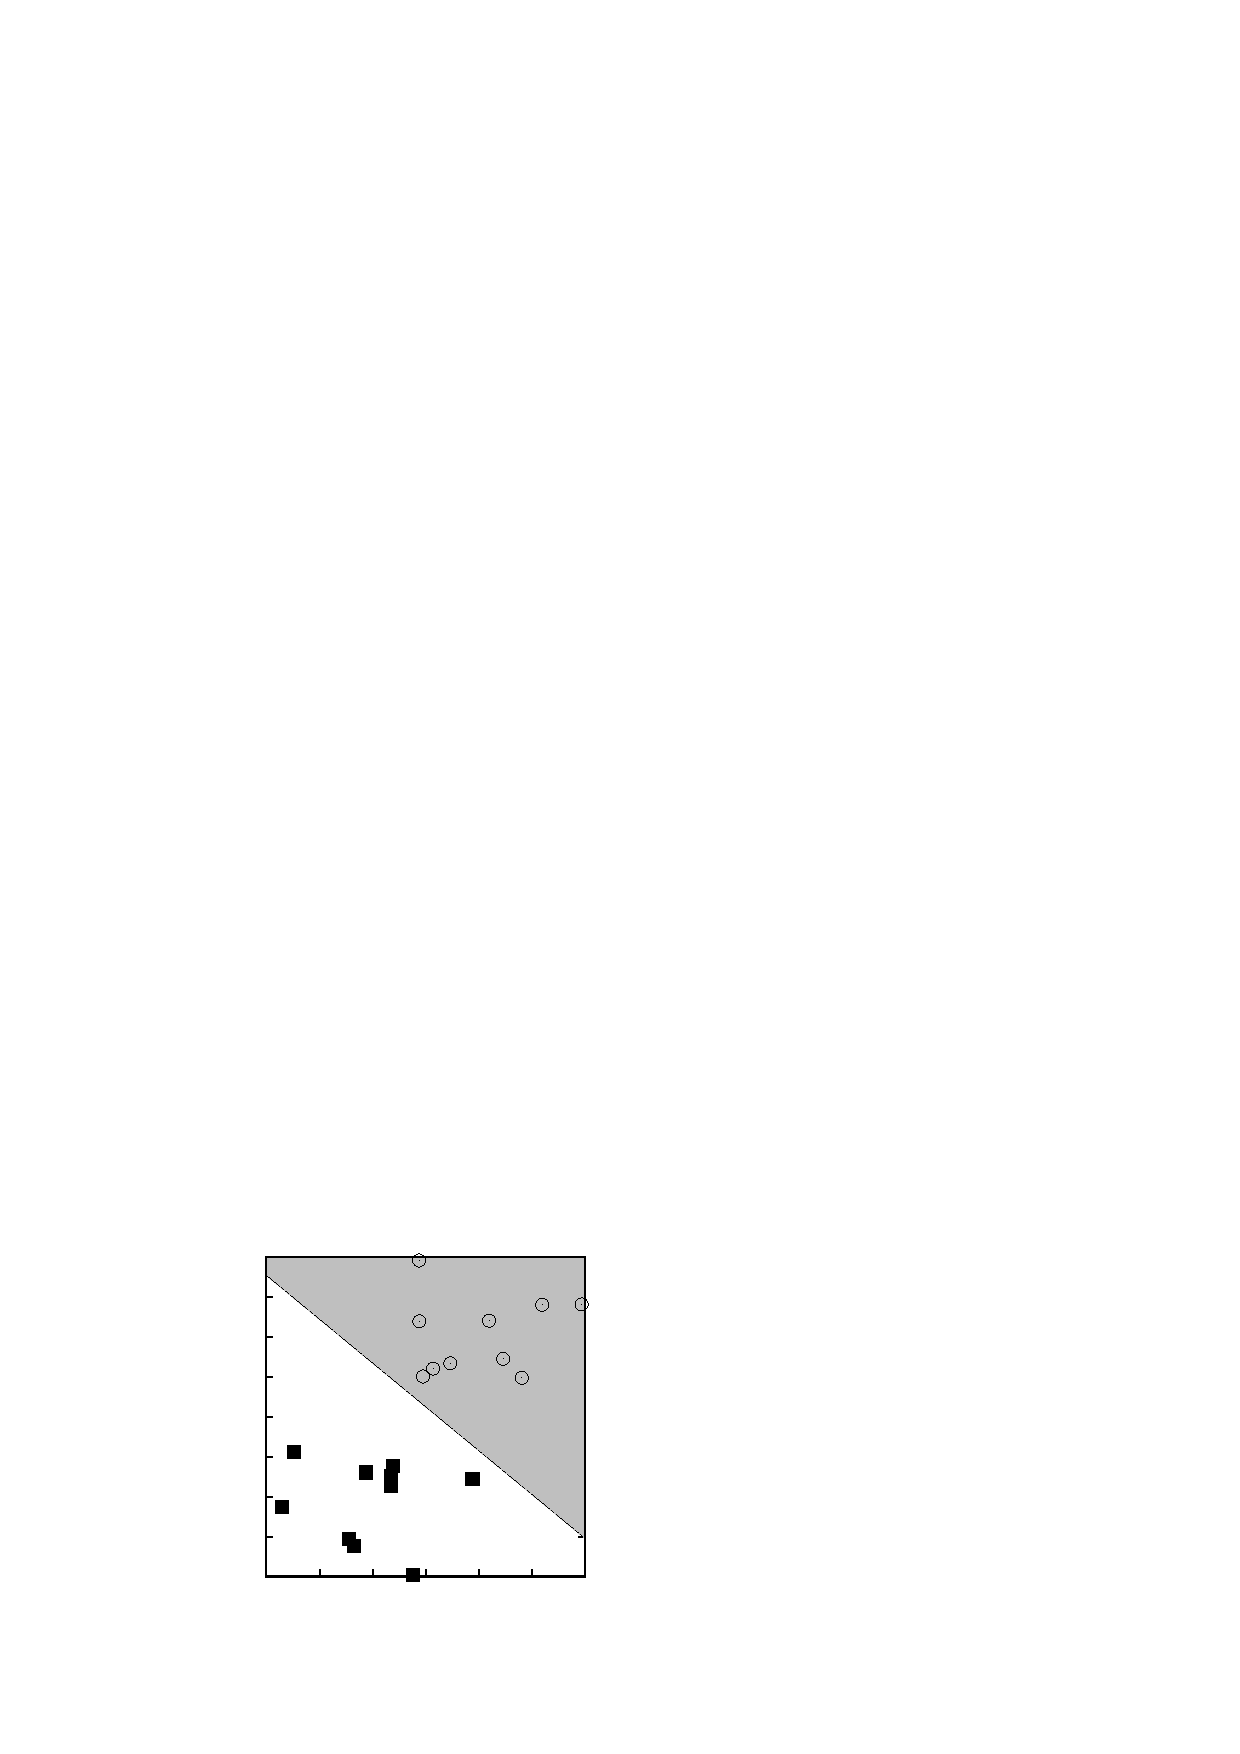
\includegraphics{linear_classifier.png}
\end{center}
}
\caption{Here the shaded region corresponds to $1.1x_1+x_2>0.25$, so
  if $w_1=1.1$ and $w_2=1$ with $\theta=0.25$ then the corresponding
  perceptron neuron will be one for all the circle points and -1 for
  all the square points.\label{fig:linear_classifier}}
\end{figure}


\begin{figure}
  \ifthenelse{\boolean{nopics}}
               {{\textsl{In the figure the line $1.1x_1+x_2=0.25$ divides the plane into two halves, there are ten randomly placed red points one side of the line, ten randomly placed blue points the other. There are three additional dotted lines close to the main $1.1x_1+x_2=0.24$, these lines also separate the points in a red group and a blue group.}}}
                            {
\begin{center}  
  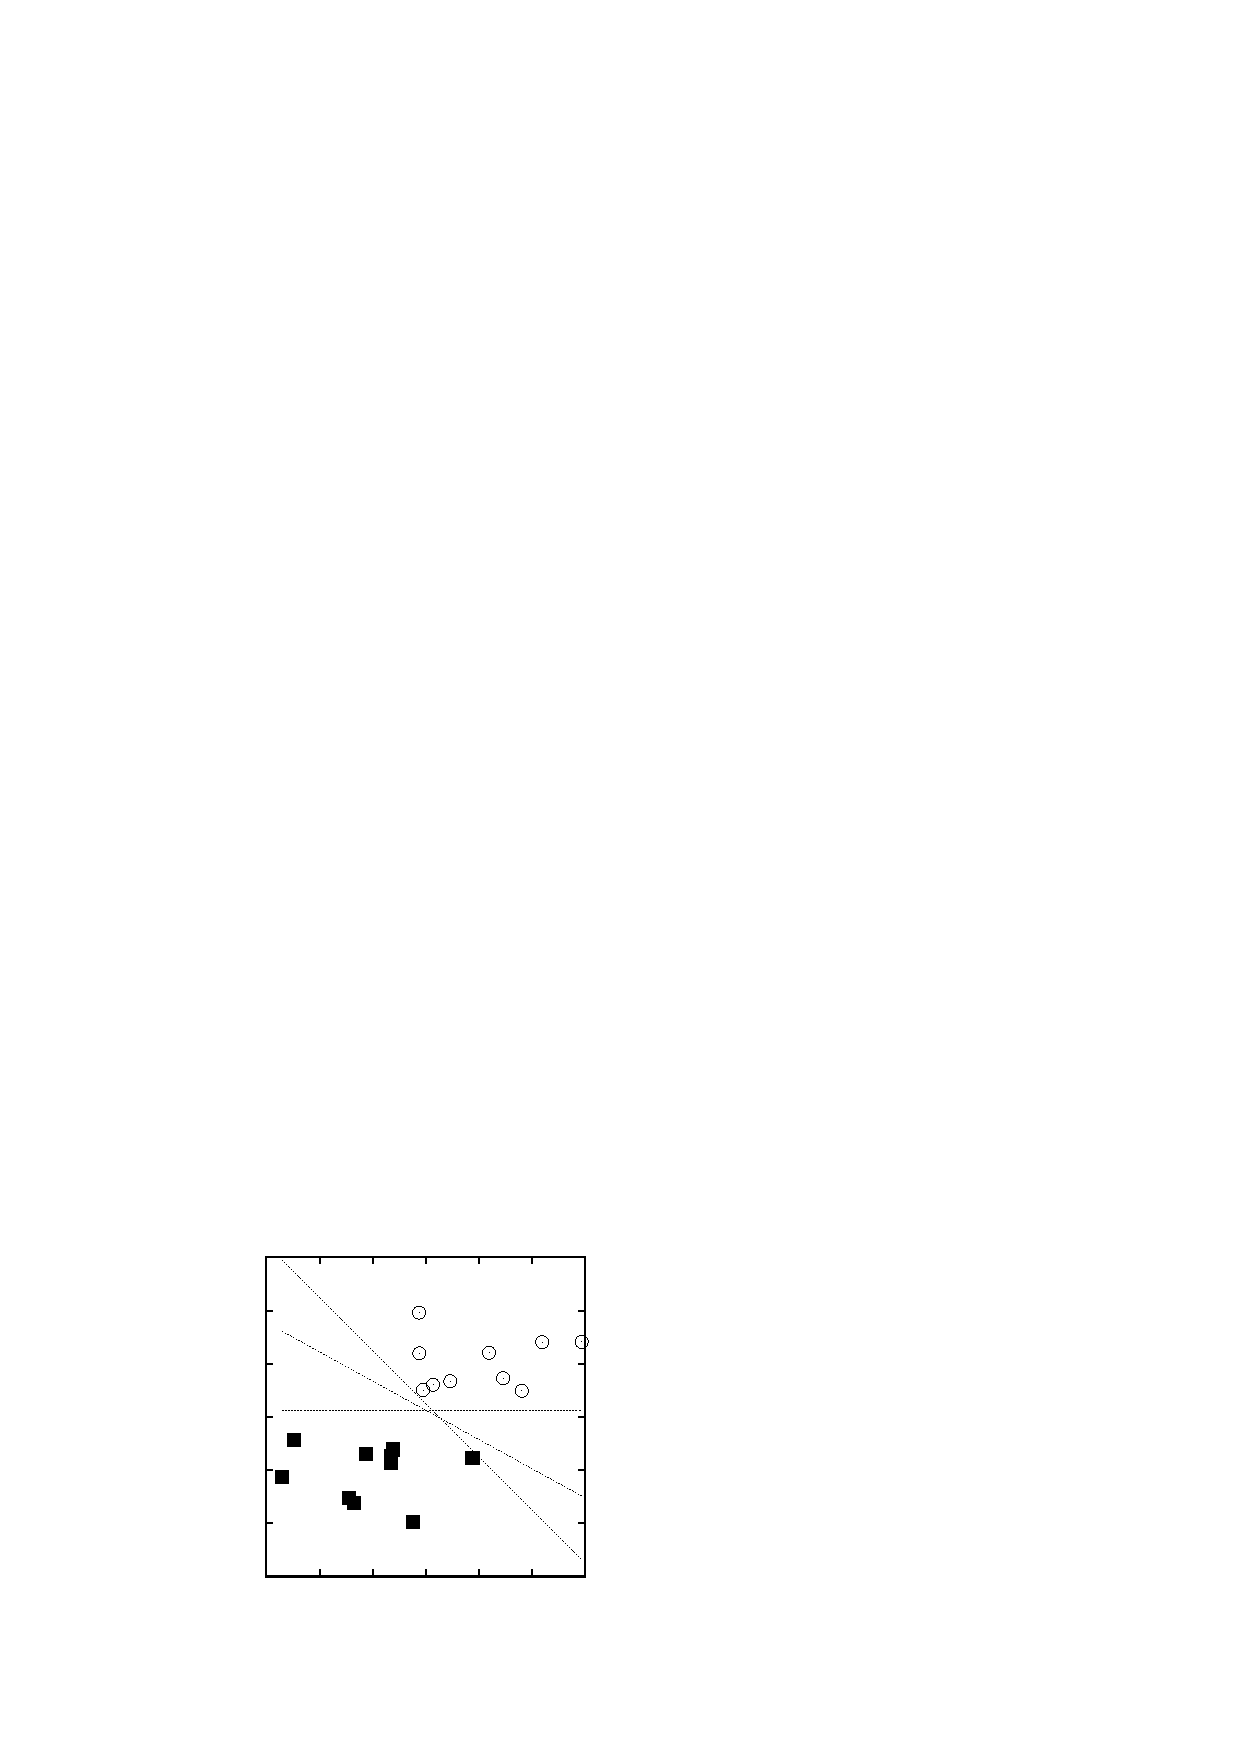
\includegraphics{random_points.png}
\end{center}
}\caption{All of these lines separate the points into two classes\label{fig:random_points}}
\end{figure}

The perceptron learning rule can be motivated by thinking about error
minimization. Consider an error function
\begin{equation}
E=\langle(d^a-y^a)^2\rangle_a
\end{equation}
If $a$ labels lots of input, $\textbf{x}^a$, desired output $d^a$
pairs, with $y^a$ the actual output; the angle brackets are an average
over these pairs. Now consider the gradient of $E$ with $w_{i}$:
\begin{equation}
\frac{\partial E}{\partial w_{i}}=-2\left\langle (d^a-y_a) \frac{\partial y^a}{\partial w_{i}}\right\rangle
\end{equation}
Now if we ignore for the moment the fact that the activation function for the McCulloch-Pitt neuron isn't differentiable and write
\begin{equation}
y^=\phi(r)
\end{equation}
with 
\begin{equation}
r=\sum_{i}w_i x_i-\theta
\end{equation}
we have
\begin{equation}
\frac{dy^a}{dw_i}=\frac{d\phi}{dr}\frac{\partial r}{\partial w_i}
\end{equation}
so using
\begin{equation}
\frac{\partial r}{\partial w_i}=x_i
\end{equation}
we get
\begin{equation}
\frac{\partial E}{\partial w_{i}}=-2\left\langle (d^a-y^a)x^a_i (\mbox{stuff involving the derivative of }\phi)\right\rangle
\end{equation}
Of course, in the McCulloch-Pitts case the \lq{}stuff involving the
derivative of $\phi$\rq{} is either zero or undefined, but we can that
this gives a similar learning rule: one way to reduce the error is to
move a tiny amount in the opposite direction to the gradient, the
gradient is the direction along which the value increases
quickest. The actual perceptron rule we gave updates a small bit after
every presentation rather than averaging first over a collection of
presentations, both approaches make sense. Here we have dealt with the
weights, the same approach can be applied to the threshold $\theta$.

This is the way to a more modern approach to the perceptron rule and
these days smooth, or mostly-smooth activation functions are used in
artificial neurons for this reason. The basic limitation of the
perceptron is that it has only one layer and so only learns a linear
classification; these days artificial neural networks have more than
one layer; this complicates the idea of adjusting the $w_i$ in a way
that is weighted by $x_i$, this, in a sense, changing the weight
according to how much it is \lq{}to blame\rq{} for the error. Back
propagation resolves this, it can be thought of as propagating the
error backwards from layer to layer; although another way to think of
it is as doing gradient descent on all the weights. At the moment the
back propagation algorithm is not considered very biological, though
it is very possible that when we understand why deep learning networks
are so effective it will be clear that the important aspects of the
algorithm can be recognized in neuronal dynamics.

\begin{thebibliography}{10}

\bibitem{Rosenblatt1958}
Rosenblatt, F. (1958), The Perceptron: A Probabilistic Model for Information Storage and Organization in the Brain, Cornell Aeronautical Laboratory.
\newblock Psychological Review, 65:386--408.


\end{thebibliography}

\end{document}

